\subsection{Model formulation}

I begin by introducing new notation to describe labels as observations within an HMM. If labels are modelled as observations, then it is straightforward to model how observing a label at time $t$ can depend upon both the hidden state $X_t$ and the observation $Y_t$.

In addition to a hidden state $X_t$ and observation $Y_t$, suppose that a \textit{label indicator} $L_t \in \{0,1\}$ is observed at time $t$ such that 
%
\begin{equation*}
    L_t := \onevec_{\{X_t\text{ is observed}\}}.
\end{equation*}
%
The label $L_t$ is itself an observation from the HMM, just like $Y_t$. As such, I define the \textit{augmented} observation at time $t$ as
%
\begin{equation*}
    \Ya_t := (X_t L_t, Y_t), \qquad
    \ya_t := (x_t \ell_t, y_t),
\end{equation*}
%
where $\Ya_t$ is a random variable and $\ya_t$ is a realization of that random variable. In this way, one may simply specify an HMM so that the hidden states are $X = \{X_1,\ldots,X_T\}$ and the observations are $\Ya = \{\Ya_1,\ldots,\Ya_T\}$. An HMM defined in this way obeys standard assumption that, conditioned on $X$, the set of observations $\{\Ya_1,\ldots,\Ya_T\}$ has independent components (for an HMM) or represents a Markov chain (for a CarHMM).

% introduce \thetaa here (augemented theta) %

I now describe one way to formulate the emission distributions $f$ to explicitly model the emission probability of $L_t$ conditioned on the hidden state $X_t$ and the observation $Y_t$. First, I define an augmented set of parameters for hidden state $i$ as $\thetaa^{(i)} := \{\theta^{(i)}_{\ell},\theta^{(i)}\}$, where $\theta^{(i)}_{\ell}$ parameterizes the probability mass of $L_t$ given $X_t = i$ and $Y_t$.  Then, denote the density of the emission distribution of $\Ya_t$ given $X_t = i$ as $\fa^{(i)}(\cdot,\thetaa^{(i)})$, where
%
\begin{gather}
    \fa^{(i)}(\ya_t;\thetaa^{(i)}) = f^{(i)}(y_t;\theta^{(i)}) ~ f^{(i)}(x_t\ell_t \mid y_t;\theta^{(i)}_{\ell})
    \label{eqn:PHMM_emis}, \quad \text{where: } \\
    %
    f^{(i)}(0 \mid y_t;\theta^{(i)}_{\ell}) + f^{(i)}(i \mid y_t;\theta^{(i)}_{\ell}) = 1, \qquad f^{(i)}(j \mid y_t;\theta^{(i)}_{\ell}) = 0, \enspace \text{for} \enspace j \notin \{0,i\}. \nonumber
\end{gather}
%
In words, $f^{(i)}(\cdot|y_t;\theta^{(i)}_{\ell})$ is the probability mass function of $X_t L_t$ conditioned on $Y_t = y_t$ when $X_t = i$. Note that the dependence on $X_t = i$ is encoded through the superscript of $f^{(i)}(\cdot|y_t)$ to be keep notation consistent (e.g. $f^{(i)}$, $\theta^{(i)}$, etc.). I will sometimes suppress notation and write $\fa^{(i)}(\ya_t;\thetaa^{(i)})$ simply as $\fa^{(i)}(\ya_t)$. %This distribution is similar to a standard HMM, but with the addition of $f^{(i)}(\ell_t|y_t;\theta^{(i)}) \in [0,1]$, which describes the probability of observing the hidden state $X_t$ given that $X_t = i$ and $Y_t = y_t$. Note that $f^{(i)}(\ell_t = 0|y_t) + f^{(i)}(\ell_t = 1|y_t) = 1$.
I refer to this model as a \textit{partially hidden Markov model}, or PHMM. 

As an example to  motivate the PHMM, consider an HMM used to model the behaviour of a predator with regular velocity readings as observations. Assume that there are two behavioural states (resting and hunting), where $X_t = 1$ corresponds to resting and $X_t = 2$ corresponds to hunting. Further, suppose that researchers can observe successful prey captures via a crunching sound that is registered on an acoustic recorder. Labels are never observed when the animal is resting ($X_t = 1$), so $f^{(1)}(x_t\ell_t = 1|y_t) = 0$ and $f^{(1)}(x_t\ell_t = 0|y_t) = 1$ for all observations $y_t$. 
%(recall that $f^{(1)}(0|y_t) = 1-f^{(1)}(1|y_t)$ $f^{(1)}(x_t\ell_t|y_t) = 0$ for all $x_t\ell_t \notin \{0,1\}$). 
In addition, it is reasonable to assume that the predator may be more likely to catch its prey when it is running fast, so $f^{(2)}(x_t\ell_t = 2|y_t)$ may be modelled as an increasing function of $y_t$ (say, $f^{(2)}(x_t\ell_t = 2|y_t) = \text{expit}(y_t)$). In this way, the probability of observing a label depends upon both the hidden behavioural state $X_t$ and the observation $Y_t$.

The likelihood of a PHMM is similar to a standard HMM:
%
\begin{equation}
    \calL(\thetaa,\Gamma;\ya) = \delta \Pa(\ya_1;\thetaa) \prod_{t=2}^T \Gamma \Pa(\ya_t;\thetaa) \onevec_N,
    \label{eqn:PHMM_like}
\end{equation}
%
where $\Pa(\ya;\thetaa)$ is an $N \times N$ diagonal matrix whose $(i,i)^{th}$ entry is equal to $\fa^{(i)}(\ya;\thetaa^{(i)})$ for $i = 1,\ldots,N$. Note that if $\ell_t = 1$ and $X_t = i$ then the only non-zero element of $\Pa(\ya_t;\thetaa)$ is entry $(i,i)$ since $f^{(i)}(x_t\ell_t = j|y_t;\theta^{(i)}_{\ell}) = 0$ for $j \neq i$.

The HMMs used in \citet{McClintock:2018} and \citet{Li:2021} that do not model labels as observations can be written as PHMMs. In particular, define some non-random set of observation times as $\calT$. Then, the models of \citet{McClintock:2018} and \citet{Li:2021} are equivalent to a PHMM with the following emission distributions:
%
\begin{gather}
    \fa_t^{(i)}(\ya_t) = f^{(i)}(y_t) f_t^{(i)}(x_t \ell_t|y_t) \nonumber \\
    %
    f_t^{(i)}(x_t\ell_t = i|y_t) = \begin{cases} 1, & t \in \calT \\ 0, & t \notin \calT. \end{cases} \label{eqn:PHMM_emis_niave}
\end{gather}
%
In other words, these studies assume that the probability of observing a label is either $1$ or $0$, and these probabilities are predefined by some known set $\calT$.

I argue that this formulation may miss important information if the probability of observing a label is a function of $X_t$ and/or $Y_t$. By explicitly modelling the probability of getting a label from an observation, I treat the presence or absence of a label itself as important information that can be used to model animal movement more accurately.

\subsection{Simulation study}

To explore issues that arise when data generated from a PHMM is fit using a misspecified model, I simulated $500$ data sets made up of $T = 100$ observations from a PHMM with $N = 3$ hidden states. The probability transition matrix was set to 
%
\begin{equation*}
   \Gamma = \begin{pmatrix} 
                0.8 & 0.1 & 0.1 \\
                0.1 & 0.8 & 0.1 \\
                0.1 & 0.1 & 0.8 
            \end{pmatrix}, 
\end{equation*}
%
with stationary distribution $\delta = \begin{pmatrix} 1/3 & 1/3 & 1/3 \end{pmatrix}$. 
%
The emission distributions for the data, $\{Y_t\}_{t=1}^{100}$, were set to normal distributions with densities
\begin{equation*}
    f^{(i)}(y_t) = \phi(y_t,\mu^{(i)},\sigma^{(i)2}),
\end{equation*}
where $\phi(y_t,\mu^{(i)},\sigma^{(i)2})$ is the density of a normal distribution with mean $\mu^{(i)}$ and variance $\sigma^{(i)2}$ evaluated at $y_t$. I set $\mu^{(1)} = -1$, $\sigma^{(1)} = 0.5$, $\mu^{(2)} = 0$, $\sigma^{(2)}=0.5$, $\mu^{(3)} = 1$, and $\sigma^{(3)} = 0.5$.

Finally, I set the emission distributions for the labels, $\{X_t L_t\}_{t=1}^{100}$, such that
\begin{equation*}
    f^{(1)}(x_t \ell_t = 1|y_t) = f^{(2)}(x_t \ell_t = 2|y_t) = 0 \quad \text{and} \quad f^{(3)}(x_t \ell_t = 3|y_t) = \text{expit}(-1+y_t)
\end{equation*}
In words, labels were only observed when $x_t = 3$, and the probability of observing a label was an increasing function of $y_t$. This is notable because the expected value of $y_t$ was larger for $x_t = 3$ compared to $x_t = 1$ and $x_t = 2$.

I fit three different HMMs to each simulated data set: 
%
\begin{enumerate}
    \item A traditional HMM which ignores $\ell_t$ as a data stream altogether.
    \item A PHMM which defines the label emission probability as $f_t^{(i)}(x_t \ell_t = i|y_t)$. This label emission probability is identical to that from Equation (\ref{eqn:PHMM_emis_niave}) and \cite{McClintock:2018}.
    \item A PHMM with the following label emission probabilities:
    \begin{gather}
        f^{(1)}(x_t \ell_t = 1|y_t) = f^{(2)}(x_t \ell_t = 2|y_t) = 0, \enspace \text{and} \nonumber \\
        %
        f^{(3)}(x_t \ell_t = 3|y_t) = \text{expit}(\theta^{(3)}_0+\theta^{(3)}_1 y_t).
        \label{eqn:PHMM_emis_ss}
    \end{gather}
\end{enumerate}

The simulated data represents a process for which labels are observed preferentially (i.e. labels are more likely to be observed when $y_t$ is larger). The first model (model 1) represents the situation where the labels are not used at all. The second model (model 2) uses the labels but assumes that label observation times are known \textit{a priori} and does not explicitly model any dependence between $L_t$ and $X_t$ or $Y_t$. The final model (model 3) accounts for dependence between $L_t$ and $X_t$ or $Y_t$ and includes the generating process of the simulated data. In particular, the data was generated from model 3 with $\theta^{(3)}_0 = -1$ and $\theta^{(3)}_1 = 1$.

Figure (\ref{fig:EDA_PHMM}) shows scatter plots of the maximum likelihood estimates of each emission distribution for each simulated data set. Table (\ref{tbl:EDA_PHMM}) lists the average parameter estimates and root mean squared errors for each model.
%
\begin{figure}
    \centering
    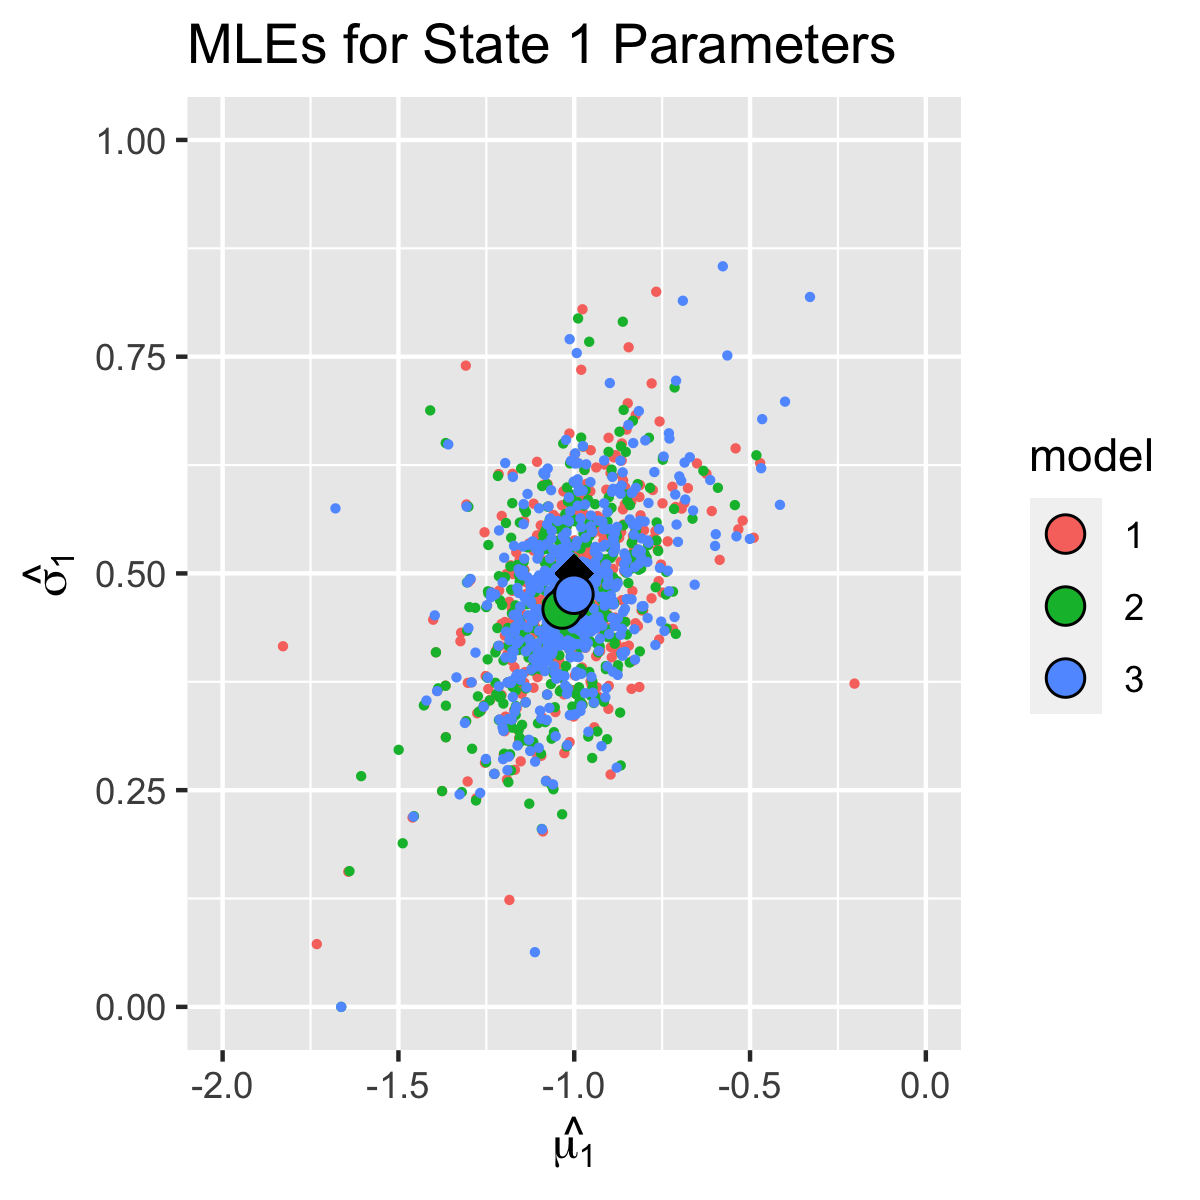
\includegraphics[width=2in]{../../src/state_1.png}
    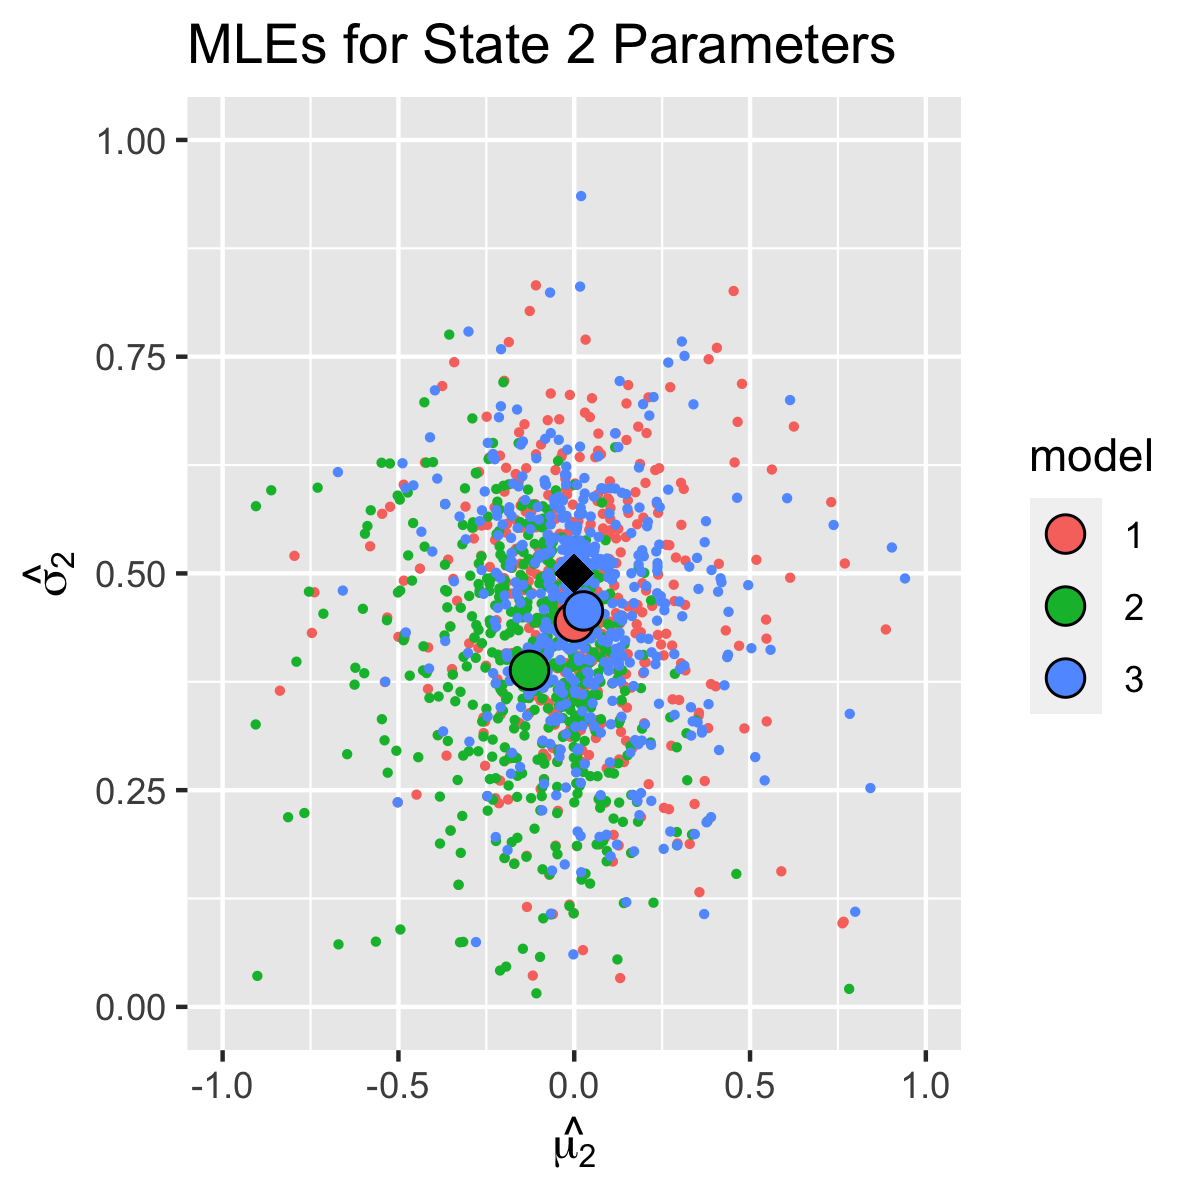
\includegraphics[width=2in]{../../src/state_2.png}
    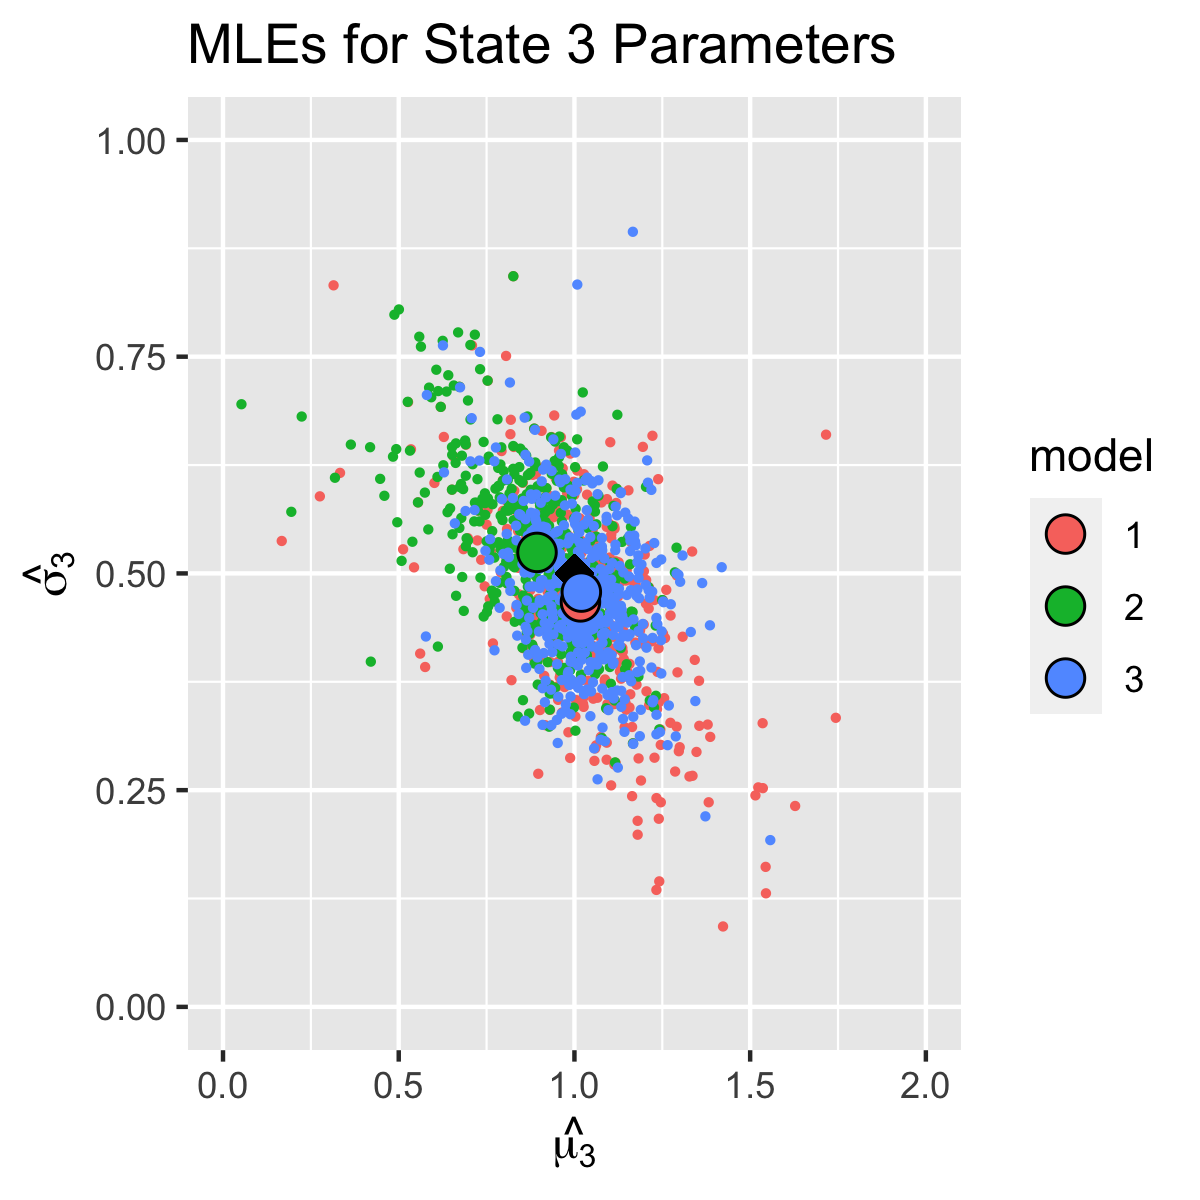
\includegraphics[width=2in]{../../src/state_3.png}
    \caption{Maximum likelihood estimates for emissions distributions of three separate PHMM. True parameters are denoted with a black diamond. Each small dot corresponds to a single MLE from a data set of length $T=100$, and the larger circles represent averages values over $500$ data sets. Model 1 is a traditional HMM, model 2 is a PHMM which models label observation times as fixed \citep{McClintock:2018}, and model 3 is a PHMM which explicitly models the label observation times as in Equation (\ref{eqn:PHMM_emis_ss}).}
    \label{fig:EDA_PHMM}
\end{figure}
%
\begin{table}
\centering
\begin{tabular}{c|cc|cc|cc}
Model & $\hat \mu^{(1)}$ & $\hat \sigma^{(1)}$ & $\hat \mu^{(2)}$ & $\hat \sigma^{(2)}$ & $\hat \mu^{(3)}$.       & $\hat \sigma^{(3)}$ \\ \hline
Truth & $-1.00$          & $0.50$              & $0.00$           & $0.50$              & $1.00$                  & $0.50$              \\
1     & $-1.01 (0.17)$   & $0.47 (0.10)$       & $0.00 (0.23)$    & $0.44 (0.15)$       & $1.02 (0.18)$           & $0.47 (0.11)$     \\
2     & $-1.03 (0.15)$   & $0.46 (0.10)$       & $-0.13 (0.26)$   & $0.39 (0.17)$       & $0.89 (0.21)$           & $0.52 (0.10)$     \\
3     & $-1.00 (0.16)$   & $0.48 (0.10)$       & $0.03 (0.21)$    & $0.46 (0.13)$       & $1.02 (\mathbf{0.13})$  & $0.48 (0.09)$
\end{tabular}
\caption{Maximum likelihood parameter estimates from model 1 (HMM without labels), model 2 (PHMM treating label observation times as fixed), and model 3 (PHMM treating label observation times as random). Parentheses refer to the average root mean squared error for each parameter estimate.}
\label{tbl:EDA_PHMM}
\end{table}
%
Model 1 and model 3 give similar \textit{average} MLE estimates for all parameters, which seems to imply that the two models are similar. However, all parameter estimates associated with model 3 have the lowest average root mean squared error among the three models. This effect is especially pronounced for $\hat \mu^{(3)}$, whose average root mean squared error is approximately 30\% lower for model 3 compared to the other two models. 
%Model 3 makes use of labels for hidden state 3, which can refine parameter estimates, so the relative accuracy of $\hat \mu^{(3)}$ makes sense. 
Model 2 produces poor parameter estimates compared to model 1 and model 3. In particular, model 2 tends to overestimate $\sigma^{(3)}$ and underestimate $\mu^{(2)}$, $\sigma^{(2)}$, and $\mu^{(3)}$. It is interesting that model 2 tends to \textit{underestimate} $\mu^{(3)}$ because labels are more likely to be observed for \textit{large} values of $y_t$. This counter-intuitive result highlights that model misspecification can affect parameter estimates in unexpected ways. In addition, the fact that model 2 produced poorer estimates than model 1 leads to the surprising conclusion that using mis-specified labels can be worse than not using labels at all. I hypothesize that performance of model 3 relative to model 1 will become better as the probability of label observation increases. I also predict that the performance of model 2 relative to model 3 will deteriorate as the dependence between $L_t$ and $X_t$ or $Y_t$ grows stronger. Testing this hypothesis formally is an area of further work for my thesis.